\section{Usage and limitation}
We test the Transfer System with 900 million $J/\psi$ data 
which takes about 5TB disk space. 
These data are divided into 9 datasets.
It took 5 days to transfer 
these data from IHEP to JINR. The throughput is shown in 
figure \ref{fig:throughput}.
\begin{figure}[h]
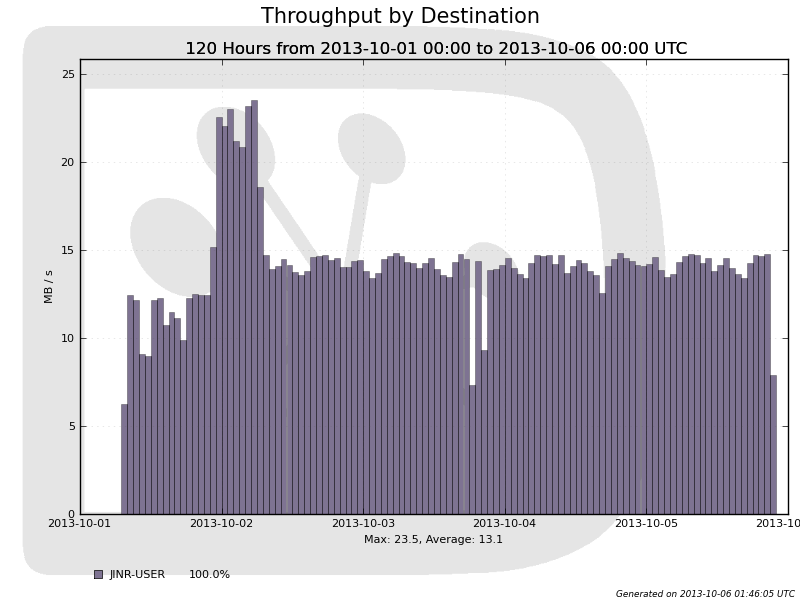
\includegraphics[width=.6\textwidth, keepaspectratio]{data/throughput-dest-1001-10-06.png}
\begin{minipage}[b]{.4\textwidth}
    \caption{\label{fig:throughput}Throughput from Oct.1 to Oct.6, 
    average throughput is 15MB/s. This figure is generated in 
{\tt DIRAC} web portal automatically.}
\end{minipage}
\end{figure}

The main limitation of this system is the inefficiency
because of the polling to check the status of the transfer processes.
It may waste some CPU time. But this system is easy to extend.
Several transfer agents can be setup in several servers.
We will test this after several {\tt DIRAC} instances are installed.

